

\begin{center}
\Huge
Funktionstyper i Maple
\end{center}

\section*{Stykvist definerede funktioner.}
\stepcounter{section}

Skal vi definere stykvist definerede funktioner i Maple, kan vi gøre det på to måder. Vi betragter et eksempel, der viser begge metoder.
\begin{exa}
	En stykvist defineret funktion $f$ er givet ved
	\begin{align*}
		f(x) = 
		\begin{cases}
			x^2 - 4 \ &\textnormal{hvis }x < 3,\\
			-2x + 11 \ &\textnormal{hvis }x \geq 3.
		\end{cases}
	\end{align*}
	Skal vi definere denne funktion i Maple, skal vi skrive følgende
	\begin{align*}
		&\texttt{restart}\\
		&\texttt{with(Gym):}\\
		&\texttt{f(x):=piecewise(x<3,x}^\texttt{2}\texttt{-4,x $\geq$ 3, -2x+11)}
	\end{align*}
	Mere generelt så skriver vi
	\begin{align*}
		\texttt{f(x):=piecewise(betingelse 1,forskrift 1,$\hdots$,betingelse n, forskrift n)}.
	\end{align*}
	Vi kan også definere en stykvist defineret funktion ved at bruge gaffelfunktionen fra paletten under \textit{expressions}.

	\begin{minipage}{0.69\textwidth}
		Vi skriver så følgende i Maple
		\begin{center}
			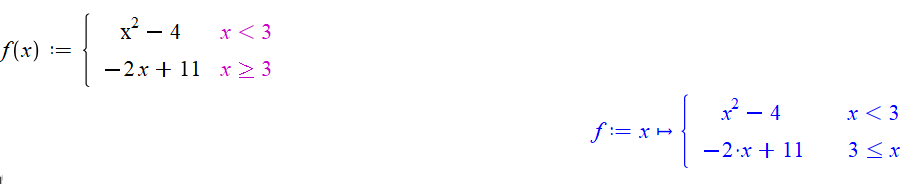
\includegraphics[width=0.9\textwidth]{Billeder/stykvisMaple}
		\end{center}
		Skal vi definere flere stykker af en funktion på denne måde, så er det blot at højreklikke (dobbeltklikke på Mac) og vælge muligheden \textit{insert row below}.
	\vspace{3cm}
	\end{minipage}
	\begin{minipage}{0.3\textwidth}
		\centering
		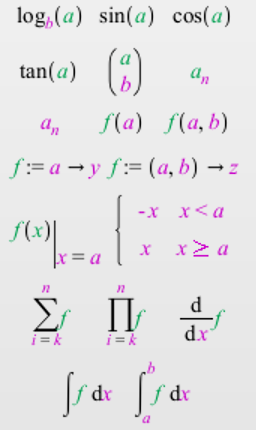
\includegraphics[width = 0.9\textwidth]{Billeder/palettestykvis}
	\end{minipage}

\end{exa}

\section*{Sammensatte funktioner i Maple}
\stepcounter{section}

Sammensatte funktioner i Maple er ganske ligetil at definere. Vi tager som før udgangspunkt i et eksempel.
\begin{exa}
	Vi betragter funktionerne $f(x) = \sqrt{x}$ og $g(x) = x^2 - 4x  + 5$. Vi ønsker at definere den 
	sammensatte funktion $h(x) = f(g(x))$ i Maple. Vi gør det som følgende
	\begin{center}
		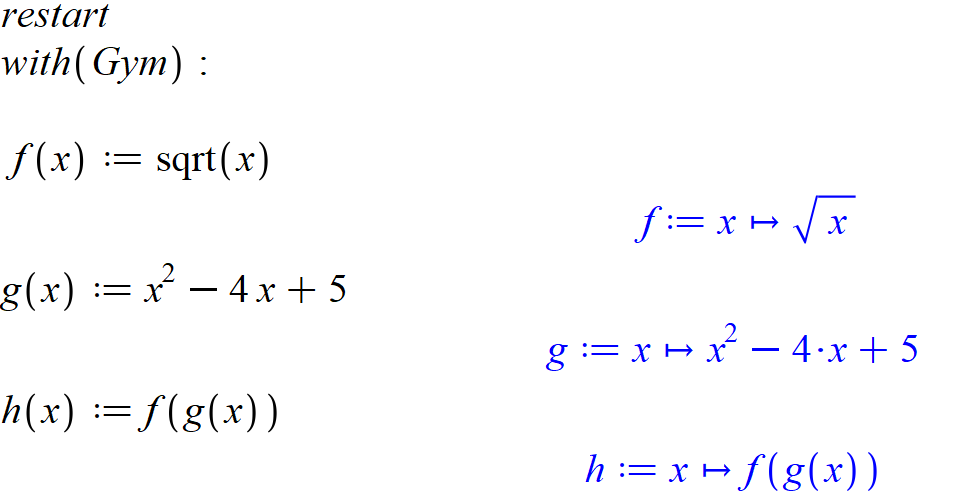
\includegraphics[width=0.6\textwidth]{Billeder/sammensatMaple}
	\end{center}
\end{exa}



\subsection*{Opgave 1}
For følgende funktioner $f$ og $g$, bestem så den sammensatte funktion $f(g(x))$ og $g(f(g))$.
\begin{align*}
&f(x) = \sqrt{x}\  \textnormal{ og } g(x) = x^2\\
&f(x) = 2x^3\  \textnormal{ og } g(x) = 10x+3\\
&f(x) = \ln(x)\  \textnormal{ og } g(x) = \frac{1}{x}\\
&f(x) = \sqrt[10]{x}\  \textnormal{ og } g(x) = x^{20}
\end{align*}
\subsection*{Opgave 2 (Maple)}
For $f(x) = x^2$ og $g(x)=2x+3$ løs ligningen
\begin{align*}
f(g(x)) = 0.
\end{align*}

\subsection*{Opgave 3}
Bestem for følgende funktion den indre og ydre funktion
\begin{align*}
	&1) \ \sqrt{2x+1}   &&2) \  2^{x^2-7}     \\
	&3) \ \frac{1}{-4x+12}   &&4) \ e^{2x-4}      \\
	&5) \ \ln(2x)   &&6) \  \log_5(7x^2)     \\
	&7) \ (x+10)^3   &&8) \  3^{\log_{10}(2x)+7}       \\
\end{align*}

\subsection*{Opgave 4}

\begin{minipage}{0.49\textwidth}
To funktioner ses på Figur \ref{fig:sammensat}. 
\begin{enumerate}[label=\roman*)]
	\item Bestem $f(-1)$.
	\item Bestem $g(0)$.
	\item Løs ligningen $f(x) = 7$.
	\item Bestem $g(f(3))$.
	\item Bestem $f(g(2))$.
	\item Løs ligningen $g(f(x)) = 6$. 
\end{enumerate}
\vspace{4cm}

\end{minipage}
\begin{minipage}{0.5\textwidth}
\begin{figure}[H]
	\centering
	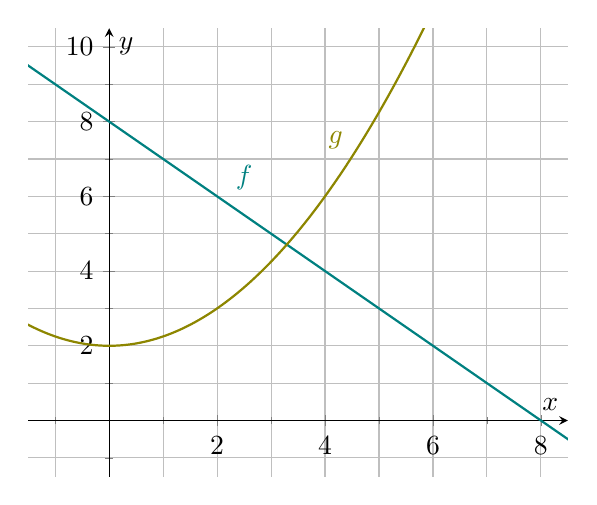
\begin{tikzpicture}
	\begin{axis}[
	axis lines = center, 
	xmin = -1.5, xmax = 8.5,
	ymin = -1.5, ymax = 10.5,
	grid = both,
	xlabel = $x$, ylabel = $y$, 
	xtick = {-4,-2,...,8,10},
	ytick = {-2,0,2,...,8,10},
	minor tick num = 1,
	]
		\addplot[color = teal, thick, domain = -2:11] {-x + 8};
		\addplot[color = olive, thick, domain = -2:11, samples = 200] {0.25*x^2+2};
		\node[color = teal] at (axis cs: 2.5,6.5) {$f$};
		\node[color = olive] at (axis cs: 4.2,7.5) {$g$};
	\end{axis}
	\end{tikzpicture}
	\caption{Grafer for funktionerne $f$ og $g$.}
	\label{fig:sammensat}
\end{figure}
\end{minipage}



\subsection*{Opgave 5}
En stykvist defineret funktion $f$ er givet ved
\begin{align*}
	f(x) = 
	\begin{cases}
		x^2, \ &\textnormal{ hvis } x \geq 0,\\
		-x^2, \ &\textnormal{ hvis } x < 0.
	\end{cases}
\end{align*}
\begin{enumerate}[label=\roman*)]
	\item Bestem $f(3).$
	\item Bestem $f(-4).$
	\item Løs ligningen $f(x) = -64$.
\end{enumerate}

\subsection*{Opgave 6 (Maple)}
Prisen for at rejse $x$ kilometer med taxafirmaet taxA kan beskrives ved funktionen $f$ givet ved
\begin{align*}
	f(x) =
	\begin{cases}
		20x + 50, \ &\textnormal{ hvis } x \leq 8, \\
		16x + 82, \ &\textnormal{ hvis } 8 < x \leq 15, \\
		12x + 142, \ &\textnormal{ hvis } 15 < x.
	\end{cases}
\end{align*}

\begin{enumerate}[label = \roman*)]
	\item Bestem prisen for at køre 10km med taxA.
	\item Afgør, hvor langt man kan køre for 250 kr.
	\item Tegn grafen for $f$ og verificér dit svar fra i) og ii).
\end{enumerate}


